% TECM Framework Detailed Architecture - TikZ Version
% Save as figures/tikz_architecture.tex and include with \input{} or compile standalone

\documentclass[tikz,border=10pt]{standalone}
\usepackage{tikz}
\usepackage{amsmath,amssymb}
\usetikzlibrary{shapes.geometric, arrows.meta, positioning, fit, calc, backgrounds, decorations.pathreplacing}

\begin{document}

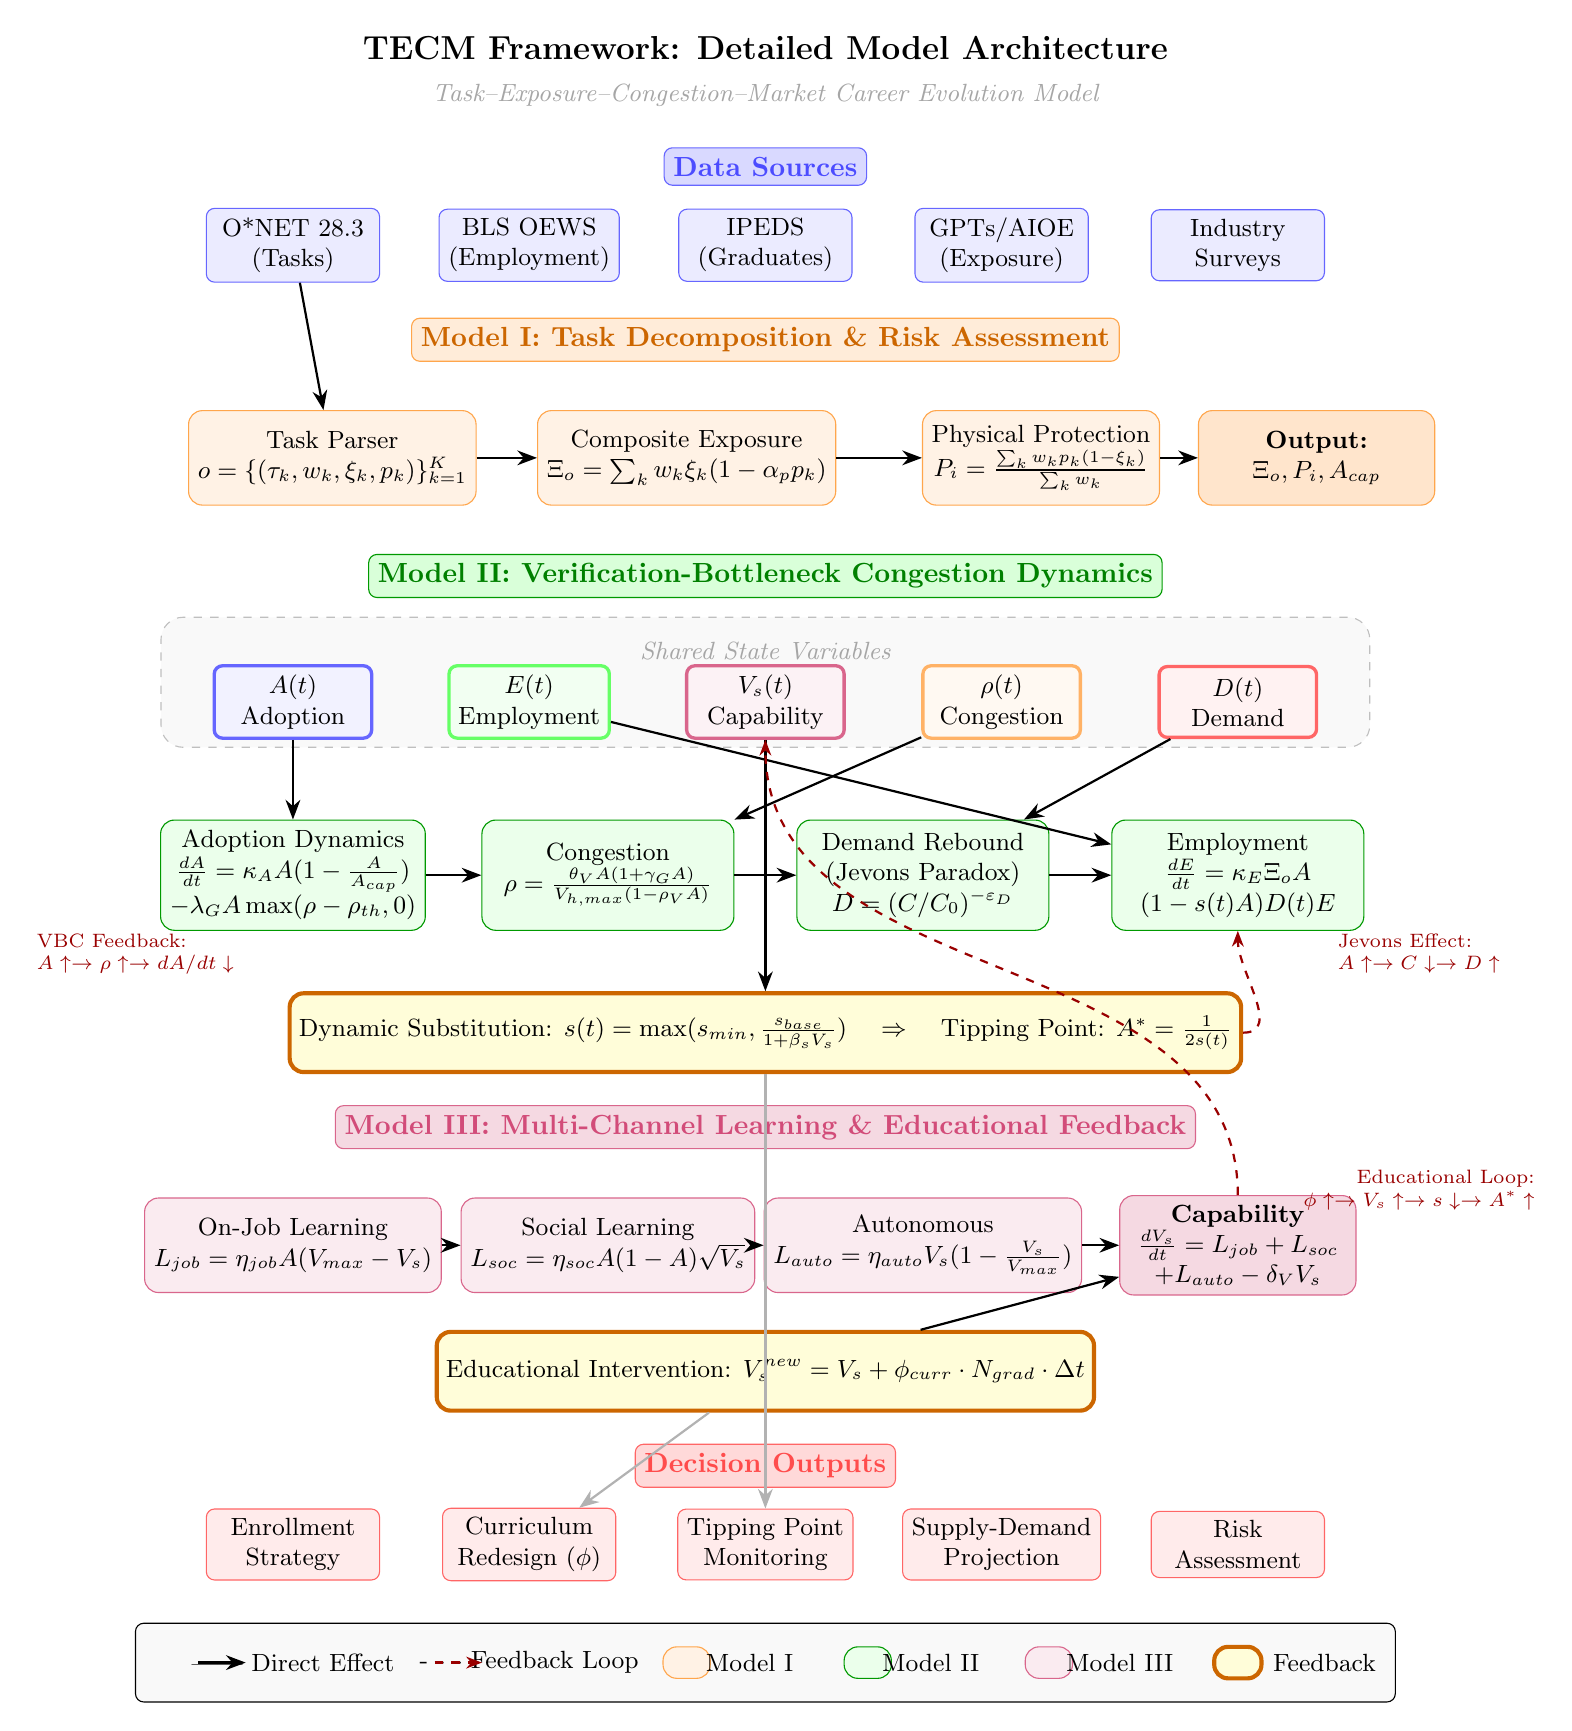
\begin{tikzpicture}[
    % Node styles
    data/.style={rectangle, rounded corners=3pt, draw=blue!60, fill=blue!8,
                 minimum height=0.8cm, minimum width=2.2cm, font=\small, align=center},
    model1/.style={rectangle, rounded corners=5pt, draw=orange!70, fill=orange!10,
                   minimum height=1.2cm, minimum width=3cm, font=\small, align=center},
    model2/.style={rectangle, rounded corners=5pt, draw=green!60!black, fill=green!8,
                   minimum height=1.4cm, minimum width=3.2cm, font=\small, align=center},
    model3/.style={rectangle, rounded corners=5pt, draw=purple!60, fill=purple!8,
                   minimum height=1.2cm, minimum width=3cm, font=\small, align=center},
    state/.style={rectangle, rounded corners=3pt, draw=gray!70, fill=white,
                  minimum height=0.9cm, minimum width=2cm, font=\small, align=center, line width=1.2pt},
    feedback/.style={rectangle, rounded corners=5pt, draw=orange!80!black, fill=yellow!15,
                     minimum height=1cm, minimum width=4cm, font=\small, align=center, line width=1.5pt},
    output/.style={rectangle, rounded corners=3pt, draw=red!60, fill=red!8,
                   minimum height=0.8cm, minimum width=2.2cm, font=\small, align=center},
    title/.style={font=\bfseries\large},
    subtitle/.style={font=\itshape\small, text=gray!70},
    section/.style={font=\bfseries, rounded corners=3pt, fill=white, draw},
    % Arrow styles
    arrow/.style={-{Stealth[length=2.5mm]}, thick},
    feedback arrow/.style={-{Stealth[length=2mm]}, thick, dashed, red!60!black},
]

% ========== TITLE ==========
\node[title] at (7.5, 16) {TECM Framework: Detailed Model Architecture};
\node[subtitle] at (7.5, 15.4) {Task--Exposure--Congestion--Market Career Evolution Model};

% ========== DATA SOURCES ==========
\node[section, draw=blue!60, fill=blue!15] at (7.5, 14.5) {\textcolor{blue!70}{Data Sources}};

\node[data] (onet) at (1.5, 13.5) {O*NET 28.3\\(Tasks)};
\node[data] (bls) at (4.5, 13.5) {BLS OEWS\\(Employment)};
\node[data] (ipeds) at (7.5, 13.5) {IPEDS\\(Graduates)};
\node[data] (aiexp) at (10.5, 13.5) {GPTs/AIOE\\(Exposure)};
\node[data] (survey) at (13.5, 13.5) {Industry\\Surveys};

% ========== MODEL I ==========
\node[section, draw=orange!70, fill=orange!15] at (7.5, 12.3) {\textcolor{orange!80!black}{Model I: Task Decomposition \& Risk Assessment}};

\node[model1] (task) at (2, 10.8) {Task Parser\\$o = \{(\tau_k, w_k, \xi_k, p_k)\}_{k=1}^K$};
\node[model1] (expo) at (6.5, 10.8) {Composite Exposure\\$\Xi_o = \sum_k w_k \xi_k (1-\alpha_p p_k)$};
\node[model1] (phys) at (11, 10.8) {Physical Protection\\$P_i = \frac{\sum_k w_k p_k (1-\xi_k)}{\sum_k w_k}$};
\node[model1, fill=orange!20] (m1out) at (14.5, 10.8) {\textbf{Output:}\\$\Xi_o, P_i, A_{cap}$};

% Model I arrows
\draw[arrow] (onet) -- (task);
\draw[arrow] (task) -- (expo);
\draw[arrow] (expo) -- (phys);
\draw[arrow] (phys) -- (m1out);

% ========== MODEL II ==========
\node[section, draw=green!60!black, fill=green!15] at (7.5, 9.3) {\textcolor{green!50!black}{Model II: Verification-Bottleneck Congestion Dynamics}};

% State variables
\begin{scope}[on background layer]
    \node[draw=gray!50, dashed, rounded corners=8pt, fill=gray!5,
          fit={(0,7.3) (15,8.6)}, inner sep=5pt] (statebox) {};
\end{scope}
\node[subtitle] at (7.5, 8.35) {Shared State Variables};

\node[state, draw=blue!60, fill=blue!5] (A) at (1.5, 7.7) {$A(t)$\\Adoption};
\node[state, draw=green!60, fill=green!5] (E) at (4.5, 7.7) {$E(t)$\\Employment};
\node[state, draw=purple!60, fill=purple!5] (Vs) at (7.5, 7.7) {$V_s(t)$\\Capability};
\node[state, draw=orange!60, fill=orange!5] (rho) at (10.5, 7.7) {$\rho(t)$\\Congestion};
\node[state, draw=red!60, fill=red!5] (D) at (13.5, 7.7) {$D(t)$\\Demand};

% Dynamics equations
\node[model2] (adopt) at (1.5, 5.5) {Adoption Dynamics\\$\frac{dA}{dt} = \kappa_A A(1-\frac{A}{A_{cap}})$\\$- \lambda_G A \max(\rho-\rho_{th},0)$};
\node[model2] (cong) at (5.5, 5.5) {Congestion\\$\rho = \frac{\theta_V A(1+\gamma_G A)}{V_{h,max}(1-\rho_V A)}$};
\node[model2] (demand) at (9.5, 5.5) {Demand Rebound\\(Jevons Paradox)\\$D = (C/C_0)^{-\varepsilon_D}$};
\node[model2] (employ) at (13.5, 5.5) {Employment\\$\frac{dE}{dt} = \kappa_E \Xi_o A$\\$(1-s(t)A)D(t)E$};

% Dynamic sub_ratio (feedback highlight)
\node[feedback] (subratio) at (7.5, 3.5) {Dynamic Substitution: $s(t) = \max(s_{min}, \frac{s_{base}}{1+\beta_s V_s})$ \quad $\Rightarrow$ \quad Tipping Point: $A^* = \frac{1}{2s(t)}$};

% Model II arrows
\draw[arrow] (A) -- (adopt);
\draw[arrow] (rho) -- (cong);
\draw[arrow] (D) -- (demand);
\draw[arrow] (E) -- (employ);
\draw[arrow] (adopt) -- (cong);
\draw[arrow] (cong) -- (demand);
\draw[arrow] (demand) -- (employ);
\draw[arrow] (Vs) -- (subratio);
\draw[feedback arrow] (subratio) to[out=0, in=-90] (employ);

% ========== MODEL III ==========
\node[section, draw=purple!60, fill=purple!15] at (7.5, 2.3) {\textcolor{purple!70}{Model III: Multi-Channel Learning \& Educational Feedback}};

\node[model3] (Ljob) at (1.5, 0.8) {On-Job Learning\\$L_{job} = \eta_{job} A(V_{max}-V_s)$};
\node[model3] (Lsoc) at (5.5, 0.8) {Social Learning\\$L_{soc} = \eta_{soc} A(1-A)\sqrt{V_s}$};
\node[model3] (Lauto) at (9.5, 0.8) {Autonomous\\$L_{auto} = \eta_{auto} V_s(1-\frac{V_s}{V_{max}})$};
\node[model3, fill=purple!15] (capability) at (13.5, 0.8) {\textbf{Capability}\\$\frac{dV_s}{dt} = L_{job}+L_{soc}$\\$+L_{auto}-\delta_V V_s$};

% Educational intervention
\node[feedback] (edu) at (7.5, -0.8) {Educational Intervention: $V_s^{new} = V_s + \phi_{curr} \cdot N_{grad} \cdot \Delta t$};

% Model III arrows
\draw[arrow] (Ljob) -- (Lsoc);
\draw[arrow] (Lsoc) -- (Lauto);
\draw[arrow] (Lauto) -- (capability);
\draw[arrow] (edu) -- (capability);
\draw[feedback arrow] (capability) to[out=90, in=-90] (Vs);

% ========== FEEDBACK LOOPS (annotations) ==========
\node[font=\scriptsize, text=red!60!black, align=left] at (-0.5, 4.5)
    {VBC Feedback:\\$A\uparrow \to \rho\uparrow \to dA/dt\downarrow$};
\node[font=\scriptsize, text=red!60!black, align=left] at (15.8, 4.5)
    {Jevons Effect:\\$A\uparrow \to C\downarrow \to D\uparrow$};
\node[font=\scriptsize, text=red!60!black, align=right] at (15.8, 1.5)
    {Educational Loop:\\$\phi\uparrow \to V_s\uparrow \to s\downarrow \to A^*\uparrow$};

% ========== OUTPUT ==========
\node[section, draw=red!60, fill=red!15] at (7.5, -2) {\textcolor{red!70}{Decision Outputs}};

\node[output] (out1) at (1.5, -3) {Enrollment\\Strategy};
\node[output] (out2) at (4.5, -3) {Curriculum\\Redesign ($\phi$)};
\node[output] (out3) at (7.5, -3) {Tipping Point\\Monitoring};
\node[output] (out4) at (10.5, -3) {Supply-Demand\\Projection};
\node[output] (out5) at (13.5, -3) {Risk\\Assessment};

% Output arrows
\draw[arrow, gray!60] (subratio) -- (out3);
\draw[arrow, gray!60] (edu) -- (out2);

% ========== LEGEND ==========
\begin{scope}[shift={(0, -4.5)}]
    \draw[rounded corners=3pt, fill=gray!5] (-0.5, -0.5) rectangle (15.5, 0.5);
    \node[font=\small] at (1.5, 0) {—— Direct Effect};
    \draw[arrow] (0.3, 0) -- (0.9, 0);
    \node[font=\small] at (4.5, 0) {- - - Feedback Loop};
    \draw[feedback arrow] (3.3, 0) -- (3.9, 0);
    \node[model1, minimum height=0.4cm, minimum width=0.6cm] at (6.5, 0) {};
    \node[font=\small] at (7.3, 0) {Model I};
    \node[model2, minimum height=0.4cm, minimum width=0.6cm] at (8.8, 0) {};
    \node[font=\small] at (9.6, 0) {Model II};
    \node[model3, minimum height=0.4cm, minimum width=0.6cm] at (11.1, 0) {};
    \node[font=\small] at (12, 0) {Model III};
    \node[feedback, minimum height=0.4cm, minimum width=0.6cm] at (13.5, 0) {};
    \node[font=\small] at (14.6, 0) {Feedback};
\end{scope}

\end{tikzpicture}

\end{document}
